\documentclass{beamer}
\beamertemplatenavigationsymbolsempty
\usepackage[french]{babel}
\usepackage{fontspec}
\usepackage{amsmath, amsthm, amsfonts}
\usepackage[separate-uncertainty]{siunitx}
\usepackage{xcolor}
\usepackage{tikz}
\usepackage{tikz-cd}
\usepackage[object=vectorian]{pgfornament}
\usepackage{circuitikz}
\usepackage{hyperref}
\usepackage{caption}
\usepackage{booktabs}
\usepackage{mathtools}
\usepackage{longtable}
\usepackage[version=3]{mhchem}
\usepackage{marginnote}
\usepackage[framemethod=tikz]{mdframed}


% Paul Tol's qualitative palette
% ``bright''.https://personal.sron.nl/~pault/#sec:qualitative
\definecolor{tblue}{HTML}{4477AA}
\definecolor{tcyan}{HTML}{66CCEE}
\definecolor{tgreen}{HTML}{228833}
\definecolor{tyellow}{HTML}{CCBB44}
\definecolor{tred}{HTML}{EE6677}
\definecolor{tpurple}{HTML}{AA3377}
\definecolor{tgrey}{HTML}{BBBBBB}


% Justification for marginnotes.
\renewcommand*{\raggedleftmarginnote}{}
\renewcommand*{\raggedrightmarginnote}{}


% Styles for mdframed environments.
\newmdenv[backgroundcolor=tgreen!10,linecolor=tgreen!30]{reponsebox}
\newmdenv[backgroundcolor=tyellow!10,linecolor=tyellow!30]{diapobox}
\newmdenv[backgroundcolor=tred!10,linecolor=tred!30]{fondamentalbox}

% Default arrow for tikz and style for positive and negative objects.
\tikzset{>=latex,
    negative/.style={draw=teal!70!black, fill=teal!10, thick},
    positive/.style={draw=red, fill=red!10, thick}}
\usetikzlibrary{matrix,calc,decorations.pathreplacing,decorations.pathmorphing,decorations.markings}

% French locale for numbers and negative exponent for units.
\sisetup{locale=FR, per-mode=symbol}

\newcommand{\abs}[1]{\left| #1 \right|}
\newcommand{\rhat}{\vec{\hat{r}}}
\newcommand{\xhat}{\vec{\imath}}
\newcommand{\yhat}{\vec{\jmath}}
\newcommand{\zhat}{\vec{k}}
\newcommand{\real}{\mathbb{R}}
\newcommand{\der}[2]{\frac{\mathrm{d}#1}{\mathrm{d}#2}}
\newcommand{\pder}[2]{\frac{\partial\ #1}{\partial\ #2}}
\newcommand{\dif}{\mathrm{d}}
\newcommand{\ddif}{\,\mathrm{d}}
\newcommand{\grad}{\vec{\nabla}}
\newcommand{\exemple}[1]{\begin{fullwidth}#1\end{fullwidth}}
\newcommand{\norm}[1]{\lVert\ #1\ \rVert}
\newcommand{\vu}{\vec{u}}
\newcommand{\vv}{\vec{v}}
\newcommand{\vr}{\vec{r}}
\newcommand{\va}{\vec{a}}
\newcommand{\vF}{\vec{F}}
\newcommand{\vE}{\vec{E}}
\newcommand{\vB}{\vec{B}}
\newcommand{\vecxyz}[3]{#1 \xhat\ + #2 \yhat\ + #3 \zhat}
\newcommand{\vecxy}[2]{#1 \xhat\ + #2 \yhat}
\newcommand{\coulombcst}{k}
\newcommand{\emf}{\ensuremath{\mathcal{E}}}
\newcommand{\eval}{\SI{1.602e-19}{C}}
\newcommand{\kval}{\SI{8.99e9}{Nm^2 \per C^2}}

% Nice separator line
\newcommand{\sectionline}{
    \noindent
    \begin{center}
        \resizebox{0.5\linewidth}{1ex}
    {{%
    {\begin{tikzpicture}
    \node  (C) at (0,0) {};
    \node (D) at (9,0) {};
    \path (C) to [ornament=85] (D);
    \end{tikzpicture}}}}
    \end{center}
}

\theoremstyle{definition}
\newtheorem*{defn}{Definition}


\usepackage[version=3]{mhchem}

\definecolor{UniBlue}{RGB}{83,121,170}
\setbeamercolor{title}{fg=UniBlue}
\setbeamercolor{frametitle}{fg=UniBlue}
\setbeamercolor{structure}{fg=UniBlue}

\begin{document}

\begin{frame}
  \frametitle{Attraction par induction dans un conducteur}
  \begin{center}
    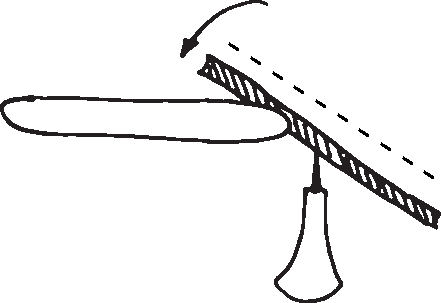
\includegraphics[scale=0.5]{../figures/tige-chargee.pdf}
  \end{center}
  \vspace{0.5cm}

  \begin{enumerate}
    \item 
\includegraphics[scale=0.5]{../figures/tige.pdf}
      \hspace{-1.3cm}\tikz \node at (-10, 0) {$---$};
    \item 
\includegraphics[scale=0.5]{../figures/tige.pdf}
      \hspace{-1.3cm}\tikz \node at (-10, 0) {$+++$};
      \hspace{-2.8cm}\tikz \node at (-10, 0) {$+++$};
    \item 
\includegraphics[scale=0.5]{../figures/tige.pdf}
      \hspace{-1.3cm}\tikz \node at (-10, 0) {$---$};
      \hspace{-2.8cm}\tikz \node at (-10, 0) {$+++$};
    \item 
\includegraphics[scale=0.5]{../figures/tige.pdf}
      \hspace{-1.3cm}\tikz \node at (-10, 0) {$+++$};
    \item<alert@2> 
\includegraphics[scale=0.5]{../figures/tige.pdf}
      \hspace{-1.3cm}\tikz \node at (-10, 0) {$+++$};
      \hspace{-2.8cm}\tikz \node at (-10, 0) {$---$};
  \end{enumerate}
\end{frame}


\begin{frame}
  \frametitle{Conservation de la charge}

  Indiquez si chacune des réactions suivantes est possible.

  \begin{enumerate}
    \item \ce{H^+ + OH^- -> H_2O} \only<2>{\alert{oui}}
    \item $\pi^+ + p^+ \longrightarrow \Sigma^0 + K^+$ \only<2>{\alert{non}}
    \item \ce{^4_2He^{2+} + ^14_7N -> ^17_8O + p^+} \only<2>{\alert{non}}
  \end{enumerate}
\end{frame}

\begin{frame}{Quantification de la charge}
  Est-ce qu'un objet peut avoir les charges suivantes?
  \begin{enumerate}
    \item $q_1 = \SI{-2.05056e-17}{C}$ \only<2>{\alert{oui}}
    \item $q_2 = \SI{3.74868e-18}{C}$ \only<2>{\alert{non}}
    \item $q_3 = \SI{4.00}{C}$ \only<2>{\alert{oui}}
  \end{enumerate}
\end{frame}

\begin{frame}[t]{Exercice}
  Deux objets métalliques identiques ont des charges $Q$ et $-6Q$,
  respectivement. Les deux objets sont mis en contact puis sont séparés.
  Quelles sont les charges sur chacun des objets?

  %\vspace{1cm}
  %\only<2>{\alert{La charge totale au début est $Q + -6Q = -5Q$. Par le
  %principe de conservation de la charge, elle devra être de $-5Q$ à la fin.
  %Puisque les deux objets sont identiques, les charges se distribueront
  %également lors du contact donc chaque objet aura la moitié de la charge
  %totale, soit $-2.5Q$.}}
\end{frame}

\begin{frame}{Électroscope}
  Que se passe-t-il si on touche la partie du haut avec une
  tige chargée négativement puis qu'on la retire?

  \begin{enumerate}
    \item Les feuillets de l'électroscope s'éloignent puis reviennent à leur
      position initiale.
    \item Les feuillets de l'électroscope se rapprochent puis reviennent à leur
      position initiale.
    \item<alert@2> Les feuillets de l'électroscope s'éloignent et demeurent éloignés.
    \item Les feuillets de l'électroscope se rapprochent et demeurent
      rapprochés.
    \item Les feuillets de l'électroscope demeurent immobiles.
  \end{enumerate}
\end{frame}


\begin{frame}{Ballon au mur}
Le coefficient de frottement entre le mur et le ballon est $0.6$, et la masse
du ballon est de \SI{2.9}{g}. Quel est
le module de la force électrique entre le ballon et le mur?
    \begin{center}
        \begin{tikzpicture}
            \draw (3, 1.7) -- (3, -1.9);
            \draw (2.298, -1.928) arc (-40:40:3);
            \draw[decorate, decoration={markings,
                mark=between positions 0 and 1 step 8mm with {
                    \node[circle, negative, minimum size=4mm] (0, 0) {$-$};}}]
            (1.915, -1.607) arc (-40:40:2.5);
            \foreach \y in {1.7, 0.9, 0.1, -0.7, -1.5} {
                \draw[positive] (3.7, \y) arc (90:270:0.5 and 0.3) -- (3.7, \y);
                \node at (3.5, \y - 0.3) {$+$};
                \draw[negative] (3.71, \y - 0.6) arc (-90:90:0.5 and 0.3) -- (3.71, \y - 0.6);
                \node at (3.9, \y - 0.3) {$-$};
            }
            \coordinate (origin) (0, 0);
            \draw[ultra thick, ->] (origin) -- (-1, 0) node[left] {$\vec{N}$};
            \draw[ultra thick, ->] (origin) -- (1, 0) node[right] {$\vec{F}_e$};
            \draw[ultra thick, ->] (origin) -- (0, 1.4) node[right] {$\vec{f}$};
            \draw[ultra thick, ->] (origin) -- (0, -1.4) node[right] {$\vec{F}_g$};
            \draw[draw=white,fill=white] (-0.02, -0.02) rectangle (0.02, 0.02);
            \node at (-1, 1.7) {Ballon};
            \node at(6, 1.7) {Mur};
        \end{tikzpicture}
    \end{center}
\end{frame}


\begin{frame}{Coulomb 1D}
  Deux charges immobiles $q_1 = \SI{4.00}{nC}$ et $q_2 = \SI{-6.00}{nC}$ sont
  situées à \SI{5}{cm} l'une de l'autre.
  Est-il possible de placer une troisième charge le long de la droite reliant
  $q_1$ et $q_2$ de telle sorte qu'elle soit à l'équilibre?
\end{frame}


\begin{frame}{Coulomb 2D}
  On considère l'ensemble de charges représenté ci-dessous. Les charges sont
  immobiles.

  \begin{center}
  \begin{tikzpicture}[scale=1]
    \node[circle, positive] at (0, 2) (q1) {$q_1$};
    \node[circle, positive] at (0, 0) (q2) {$q_2$};
    \node[circle, positive] at (5, 0) (q3) {$q_3$};
    \node[circle, positive] at (5, 2) (q4) {$q_4$};
    \draw[<->] (q1) -- node[fill=white] {$l$} (q2);
    \draw[<->] (q2) -- node[fill=white] {$d$} (q3);
  \end{tikzpicture}
  \end{center}

  \begin{enumerate}
    \item Trouver une expression algébrique qui représente la force
      électrostatique nette exercée sur la charge $q_4$.
    \item Si $q_1 = \SI{32.8}{nC}$, $q_2 = \SI{1.34}{\micro C}$, $q_3 =
      \SI{-234}{nC}$, $q_4 = \SI{78.6}{nC}$, $l = \SI{0.314}{mm}$ et $d =
      \SI{2.13}{mm}$, déterminer la force électrostatique nette exercée sur la
      charge $q_4$.
  \end{enumerate}
\end{frame}



\begin{frame}{Énigme}
  On place une particule chargée à l'intérieur d'une sphère métallique creuse.
  À proximité, on place un pendule dont l'extrémité est métallique. Que se
  passe-t-il?

  \uncover<2>{
  \begin{center}
    \begin{tikzpicture}
      \draw[orange, fill=orange!20] (4, 1.5) -- (4, 0) -- (5, 0) -- (5, 1.5);
      \draw[ultra thick, fill=white] (4.5, 2) circle[radius=1];
      \node[circle, draw=black!70, fill=black!10] at (4.5, 2.0) {$+$};
      \node[circle, draw=black!80, fill=black!40, minimum size=6mm] (bob)
        at (0.7, 2.2) {};
      \draw[ultra thick] (-1.5, 0) -- (-1.5, 3) -- (0, 3);
      \draw (0, 3) -- (bob);
      \node at ($(bob) + (0.15, 0.13)$) {$-$};
      \node at ($(bob) + (0.15, -0.13)$) {$-$};
      \node at ($(bob) + (-0.15, 0.13)$) {$+$};
      \node at ($(bob) + (-0.15, -0.13)$) {$+$};
      \draw[decorate, decoration={markings,
                      mark=between positions 0 and 1 step 5.1mm with {
                         \node (0, 0) {$-$};}}] (4.5, 2) circle[radius=0.8];
      \draw[decorate, decoration={markings,
                      mark=between positions 0 and 1 step 6mm with {
                         \node (0, 0) {$+$};}}] (4.5, 2) circle[radius=1.2];
    \end{tikzpicture}
  \end{center}
  }
\end{frame}

\end{document}
